\documentclass{report}
\usepackage[utf8]{inputenc} %encodage entrée
\usepackage[T1]{fontenc}
\usepackage{graphicx} %images
\usepackage[usenames,dvipsnames]{xcolor} %couleurs
\usepackage{tikz} %schémas
\usetikzlibrary{calc}
\usepackage{tikz-uml}
\usepackage{pgfgantt}
\usepackage[chapter]{minted} %mise en forme de code source
\usepackage{framed} %cadres et bordures
\usepackage[frenchb]{babel} %langue
\usepackage{amsmath} %symboles maths
\usepackage{caption} %legendes
\usepackage{subcaption} %légendes et sous-figures
\usepackage{enumitem} %formatage des listes à puces
\usepackage[nobottomtitles]{titlesec} %formatage des chapitres
\usepackage{blindtext}
\usepackage[a4paper]{geometry} %mise en page
\usepackage[hidelinks]{hyperref} %liens
\usepackage{lastpage} %pagination 1/n
\usepackage{fancyhdr} %headers&footers

\usepackage{upquote}
\usepackage{textcomp}
\usepackage{minted}
\usepackage{inconsolata}
\renewcommand{\listingscaption}{Code}
\usepackage{MnSymbol}

\newminted[cppcode]{c++}{
  breaklines             = true,
  frame                  = single,
  breakautoindent        = true,
  breaksymbolleft        = $\lhookrightarrow$,
  breaksymbolindentleft  = 10pt,
  breaksymbolsepleft     = 2pt,
  breaksymbolright       = $\rhookleftarrow$,
  breaksymbolindentright = 10pt,
  breaksymbolsepright    = 2pt,
  texcomments            = true
}


\newmintedfile[cppfile]{c++}{
  linenos                = true,
  tabsize                = 2,
  breaklines             = true,
  frame                  = single,
  breakautoindent        = true,
  breaksymbolleft        = $\lhookrightarrow$,
  breaksymbolindentleft  = 10pt,
  breaksymbolsepleft     = 2pt,
  breaksymbolright       = $\rhookleftarrow$,
  breaksymbolindentright = 10pt,
  breaksymbolsepright    = 2pt,
  label                  = Code C++,
  texcomments            = false
}

\newmintinline[cppinline]{c++}{
}
\hypersetup{
  bookmarks=false,         % show bookmarks bar?
  unicode=false,          % non-Latin characters in Acrobat’s bookmarks
  pdftoolbar=false,        % show Acrobat’s toolbar?
  pdfmenubar=false,        % show Acrobat’s menu?
  pdffitwindow=false,     % window fit to page when opened
  pdfstartview={FitH},    % fits the width of the page to the window
  pdftitle={},    % title
  pdfauthor={Pierre-Loup Pissavy},     % author
  pdfsubject={},   % subject of the document
  pdfcreator={PDFLaTeX},   % creator of the document
  pdfproducer={LaTeX}, % producer of the document
  pdfnewwindow=true,      % links in new window
  colorlinks=false,       % false: boxed links; true: colored links
  linkcolor=red,          % color of internal links (change box color with linkbordercolor)
  citecolor=green,        % color of links to bibliography
  filecolor=magenta,      % color of file links
  urlcolor=cyan           % color of external links
}


\hypersetup{
  pdftitle={Projet ZZ2 - Simulation Multi-Agents}
}

%styles et formatage
\geometry{scale=0.8,centering}
\frenchbsetup{StandardLists=true}

\newcommand{\hsp}{\hspace{10pt}}
\newcommand{\TikZ}{Ti{\color{orange}\textit{k}}Z}

\newcommand{\blankpage}{\newpage \thispagestyle{empty} \addtocounter{page}{-1} \null \newpage}

\titleformat{\chapter}[hang]{\LARGE\bfseries}{\thechapter\hsp\textcolor{lightgray}{|}\hsp}{0pt}{\LARGE\bfseries}

\captionsetup[table]{name=\textsc{Tableau}}
\renewcommand{\listingscaption}{Fichier}
\renewcommand{\listoflistingscaption}{Liste des fichiers}

% Pages de contenu
\fancypagestyle{IHA-fancy-style}{%
  \fancyhf{}%
  \fancyhead[R]{\leftmark}
  \fancyfoot[R]{\thepage/\pageref{LastPage}}
  \fancyfoot[L]{Projet ZZ2 -- Simulation Multi-Agents}%
  \renewcommand{\headrulewidth}{0.4pt}% Ligne de header
  \renewcommand{\footrulewidth}{0.4pt}% Ligne de footer
}
% Style de base: sert pour les nouveaux chapitres
\fancypagestyle{plain}{%
  \fancyhf{}%
  \fancyfoot[R]{\thepage/\pageref{LastPage}}%
  \fancyfoot[L]{Projet ZZ2 -- Simulation Multi-Agents}%
  \renewcommand{\headrulewidth}{0pt}% pas de ligne de Header
  \renewcommand{\footrulewidth}{0.4pt}% ligne de footer
}
\pagestyle{IHA-fancy-style}


\begin{document}
  \begin{titlepage}
  \newcommand{\HRule}{\rule{\linewidth}{0.5mm}}
  \center
  \null{}
  \vspace{3cm}

  \textsc{\LARGE ISIMA Deuxième Année}\\[1.5cm]
  \textsc{\Large Filière Génie Logiciel}\\[0.5cm]
  \HRule \\[0.4cm]
  { \huge \bfseries  Projet de simulation Multi-Agents}\\
  \HRule \\[1.5cm]

  \begin{minipage}{0.4\textwidth}
    \begin{flushleft} \large
      Pierre CHEVALIER\\
      Pierre-Loup PISSAVY
    \end{flushleft}
  \end{minipage}
  ~
  \begin{minipage}{0.4\textwidth}
    \begin{flushright} \large
      \emph{Enseignant:} \\
      David HILL
    \end{flushright}
  \end{minipage}\\[4cm]

  {\large 2015 -- 2016}\\[3cm]

  \vfill

  
\includegraphics[width=6cm]{settings/ISIMA_logo.pdf}\\[1cm]
\end{titlepage}

  %\blankpage
  \tableofcontents
  \setlength{\parskip}{10pt}
  %\blankpage

  \chapter{Présentation}

Ce TP de Simulation s’inscrit également dans le cadre du cours d’Architectures Logicielles et Qualité. Il s’agit de concevoir un programme de simulation multi-agents. Le sujet étant libre, nous avons choisi d’imaginer un monde composé de planètes. Ces planètes appartiennent à des factions qui s’affrontent mutuellement. 

Le monde est par défaut une grille carrée de 400 cases ($20 \times 20$). On peut travailler avec une grille torique (en employant la méthode d’initialisation des voisins \cppinline{void Virtual_planet::set_neighbourhood2()} en lieu et place de \cppinline{void Virtual_planet::set_neighbourhood()}).

Le monde propose une liste d’agents en attente, et une liste des agents ayant déjà joué. Afin de définir un ordre aléatoire dans les attaques ou actions des agents, la liste des agents en attente est mélangée aléatoirement. Entre deux tours, la liste des agents ayant déjà joué est utilisée pour déterminer la liste des agents en attente du prochain tour.

Chaque planète peut choisir de mener une attaque afin d’étendre l’espace colonisé par la faction à laquelle elle appartient, ou bien de produire des richesses qui permettront une expansion ultérieure (car celle-ci a un coût).\\
Le coût d’une attaque est estimé selon le taux de défense de l’adversaire.\\
Lorsqu’une planète subit une attaque, elle peut tenter de parer à celle-ci. Cette parade est fonction des capacités de défense de la faction. Si elle n’a pas les capacités suffisantes, alors elle subit, ce qui a pour effet de réduire ses capacités de défense et le rendement de ses productions (dégâts et pertes).

Lorsque la planète n’adopte pas de comportement offensif, elle choisit de rendre son industrie plus pérenne et améliore ses productions (c’est le cas lorsque l’attaque a échoué). Les productions sont définies en fonction de l’expertise de la colonie et du taux de production de la planète (certaines planètes sont plus propices à l’activité industrielle).

Lorsqu’une planète libre est colonisée, alors elle est remplacée par une planète colonisée appartenant à la faction de l’attaquant. Si toutefois cette planète appartenait à une faction adverse, cette faction la perd et la nouvelle faction peut alors en profiter.

Lorsqu’une planète est attaquée, et qu’elle n’a pas encore joué, son action est annulée, car elle serait alors susceptible de s’en prendre à sa propre faction, ce qui est interdit.

Certaines planètes ont un statut spécial: les planètes mères. Il y a une planète mère par faction, elle agit comme une colonie, mais provoque la perte totale et définitive de la faction si jamais elle ne parvient pas à se défendre lors d’une attaque.

\newpage
Nous avons finalement retenu le diagramme de classes général suivant:
\begin{figure*}[h!]
	\centering
	\begin{tikzpicture}
  \umlemptyclass[x=0,y=5]{Monde}
  \umlemptyclass[x=4,y=5]{Planète virtuelle}
  \umlemptyclass[x=0,y=2.5]{Faction}
  \umlemptyclass[x=4,y=2.5]{Planète Colonisée}
  \umlemptyclass[x=8,y=2.5]{Planète libre}
  \umlemptyclass[x=4,y=0]{Planète mère}
  \umlemptyclass[x=0,y=0]{Faction neutre}

  \umlunicompo[mult2=1..*,pos2=0.8]{Monde}{Planète virtuelle}
  \umlunicompo[mult2=*,pos2=0.8]{Monde}{Faction}
  \umlinherit{Planète libre}{Planète virtuelle}
  \umlinherit{Planète Colonisée}{Planète virtuelle}
  \umlinherit{Planète mère}{Planète Colonisée}
  \umlinherit{Faction neutre}{Faction}
  \umluniaggreg[mult2=1,pos2=0.8]{Faction}{Planète mère}
  \umluniaggreg[mult2=1..*,pos2=0.8]{Faction}{Planète Colonisée}
\end{tikzpicture}

\end{figure*}

Pour réaliser ce projet, nous avons décidé d’avoir recours à plusieurs outils, et parfois d’utiliser différents outils pour parvenir à la même fin, ceci pour nous rendre compte des problèmes que nous pouvons rencontrer en entreprise lorsque plusieurs développeurs travaillent sur un même projet avec des outils différents. C’est pourquoi nous avons utilisé plusieurs IDE: Geany à l’ISIMA, QtCreator sur Windows et sur Linux, et Microsoft Visual Studio (2013 et 2015) sur Windows.

Chaque IDE propose différentes fonctionnalités plus ou moins pointues et faciles d’utilisation. Par exemple, QtCreator intègre de la documentation sur les objets utilisés spécifiques à Qt, ce qui permet d’avoir rapidement accès aux différentes méthodes disponibles, et ainsi se passer d’un basculement fréquent entre navigateur et environnement de développement. Visual Studio propose un outil d’analyse de la mémoire très performant lors du débogage.

Afin de déboguer le programme, nous avons eu recours aux outils intégrés aux IDE, mais aussi à ddd, puisqu’il fonctionne pour des programmes C++. Nous avions fait ce choix quand nous n’avions pas encore développé de solution graphique. Nous utilisions alors à ce moment différents éditeurs de texte dotés de quelques outils facilitant le codage (snippets). Pour vérifier que le programme ne provoquait pas de fuite mémoire, nous avons utilisé le très reconnu valgrind jusqu’à obtenir un résultat satisfaisant (aucune fuite).

Enfin, toute la documentation de notre code a été produite en utilisant les raccourcis que propose l’outil Doxygen, qui est présenté dans les dossiers en annexe. La documentation est proposée en PDF (compilé avec LaTeX) et en version web HTML. Cela permet la production d’un document de qualité, quasi interactif, et très utile pour toute personne qui n’a pas connaissance du travail réalisé dans le cadre de ce TP. Nous y avons ajouté une liste des choses qui peuvent être à faire, cela permet de montrer les possibilités de cet outil, et donc la qualité de l’information (mise en relief des informations critiques…). Par exemple, l’ordre de présentation est bien pensé: les tâches restant à faire apparaissent avant la documentation, ce qui permet de renseigner le lecteur immédiatement, et ainsi lui éviter de mener une recherche, laquelle peut être longue et fastidieuse, au coeur de la documentation.

La gestion des versions de notre projet est réalisée à l’aide de Git, outil pour lequel des plug-ins sont intégrés à l’interface de développement.

\newpage
Initialement, nous avions proposé le diagramme de Gantt suivant:
\begin{figure*}[h!]
	\begin{ganttchart}[vgrid,hgrid]{1}{12}
  \gantttitle{Séances}{12} \\
  \gantttitlelist{1,...,12}{1} \\
  \ganttgroup{Conception de base}{1}{3} \\
    \ganttbar{Création de la grille "Monde"}{1}{1} \\
    \ganttbar{Création des agents de base}{1}{1} \\
    \ganttbar{Tirage des agents à exécuter}{2}{2} \\
    \ganttbar{Planète mère et colonies}{3}{3} \\
    \ganttbar{Faction}{3}{3} \ganttnewline
  \ganttgroup{Simulation}{4}{7} \\
    \ganttbar{Création du système économique}{4}{5} \\
    \ganttbar{Création des désirs des factions (ordres etc)}{6}{7} \\
    \ganttbar{Respect des ordres}{6}{7} \ganttnewline
  \ganttgroup{Bonus !}{8}{12} \\
    \ganttbar{Spécialisation de faction}{8}{8} \\
	  \ganttbar{Technologie}{9}{9} \\
	  \ganttbar{Système de négociation}{10}{10} \\
	  \ganttbar{Système d'espionnage}{11}{11} \\
	  \ganttbar{Création de factions dissidentes}{12}{12}
\end{ganttchart}
\end{figure*}
  
  \chapter{Développement}

  Le développement du programme s’est fait en plusieurs étapes clef.

  Dans un premier temps nous avons créé les différentes classes prévues dans notre diagramme de classes UML. Ce qui implique l’écriture des headers et également des constructeurs de base tels que nous les concevions à ce moment. Nous nous sommes chargés ensuite de mettre en place l’initialisation des planètes sur la grille du monde, pour cela nous nous sommes occupés de terminer le constructeur de l’objet \texttt{world} (qui n’a presque pas changé depuis). Enfin nous avons implémenté les méthodes dont nous étions sûrs de leur nécessité comme les getters et les setters de certains champs critiques, ainsi que des convertisseurs, puisque nous savions que les objets (agents) présents dans notre grille monde allaient devoir être supprimés puis remplacés à la volée durant la simulation. Par exemple nous avons créé une méthode permettant de « convertir » un objet \texttt{Free\_planet} en un objet \texttt{Colonized\_planet} en ne prenant en paramètre que des champs critiques. Dans ce cas précis, nous donnons en paramètre une référence vers la faction de la nouvelle planète colonisée. C’est également dans cette partie que nous avons créé la fonction \texttt{scheduler()} qui parcourt les agents vivants et les fait agir. Cette partie que l’on pourrait qualifier de mise en place du système a duré pendant environ 20\% du projet.

  Après cette partie mise en place des agents dans la simulation, nous nous sommes attaqués aux méthodes \texttt{run()}, c’est-à-dire aux actions propres des agents dans la simulation que nous venions de mettre en place. Nous nous sommes donc d’abord chargés de la méthode \texttt{run()} des planètes colonisées puisque c’est la plus complexe. Nous avons réalisé à ce moment-là que des méthodes \texttt{run()} sur toutes les planètes n’étaient pas nécessaires, car il n’était pas prévu que les planètes sans faction agissent. Nous avons alors pu lancer nos premières simulations. Celles-ci nous ont révélé des erreurs non prévues, comme lors de la fin de la simulation qui renvoyait une segmentation fault à la suppression de la faction. S’en suivit donc une phase de bug fixing.

  C’est notamment à ce moment-là que nous avons décidé de donner aux objets \texttt{Free\_planet} une faction neutre pour avoir accès à plus de données. Comme celle-ci ne pouvait être créée qu’une seule fois (puisque en tant que faction fantôme, elle n’est pas un agent) nous avons décidé d’en faire un singleton. L’implémentation en elle-même des méthodes \texttt{run()} pour définir les actions des agents n’a duré que 5\% du temps du projet mais la partie bug fixing a dû durer elle 60\% du temps. En effet nous avons notamment rencontré des difficultés lors des conversions durant la simulation. Celles-ci rendaient les références des planètes voisines obsolètes. Cette mise à jour du voisinage fut la principale cause d’erreur durant le TP.

  Enfin, une fois une version stable obtenue, et des simulations concluantes nous nous sommes lancés dans la création d’une interface en Qt avec un afficheur d’images à la place des caractères ASCII afin de découvrir les possibilités de l’outil. Pour ce faire nous avons utilisé très simplement l’outil en affichant des cercles pour chaque planète de couleur différente suivant la faction. Cette fonction \texttt{display()} est appelée après chaque appel au scheduler. Nous avons également ajouté un tableau affichant les statistiques de chaque agent faction afin de voir en temps réel leur évolution. Nous avons ensuite peaufiné cet afficheur en rajoutant des images et des valeurs pour chaque planète (son économie et sa défense). Pour optimiser l’afficheur nous avons rajouté un booléen (qui n’était pas prévu à la base) sur les agents planètes déterminant si elle avait changé depuis le dernier tour (si ses valeurs ont évolué) et de ce fait si son affichage doit être mis à jour. Ce booléen est vrai à la construction des agents, ce qui fait que tout nouvel agent doit être affiché. De plus le getter de ce booléen passe automatiquement celui-ci à false en fin de traitement, de manière qu’une fois l’affichage mis à jour, celui-ci ne soit plus effectué tant que la méthode \texttt{changed()} (qui passe le booléen à true) n’a pas été appelée. Cette partie nous a permis de découvrir une erreur de référence concernant les factions puisque les valeurs affichées par le tableau étaient totalement erronées ce qui faussait également la simulation. Cette partie a duré 10\% du temps du projet.

  Pour terminer nous nous sommes chargés de modifier les valeurs de nos simulations afin de les rendre plus pertinentes. Nous avons également rajouté des constantes statiques dans nos classes permettant de contrôler plus efficacement les paramètres de notre simulation. Par exemple nous avons créé une constante \cppinline{MAX_COLONY_DEFENSE} qui définit la valeur max de défense que peut avoir une planète. Enfin nous avons terminé le développement du projet par une phase de bug fixing qui nous a notamment permis de corriger des problèmes de fuite mémoire (à l’aide de valgrind). Nos agents planètes envoyant des demandes de subvention aux agents factions, ces demandes lors de leur traitement n’étaient pas supprimées ensuite, ce qui impliquait qu’au fur et à mesure des simulations, les factions perdaient inutilement de l’argent.

  \section{Patrons de conception}

  Durant le TP, 3 patrons de conception notables ont été utilisés:
  
  \subsection{Patron composite}
  \begin{center}
    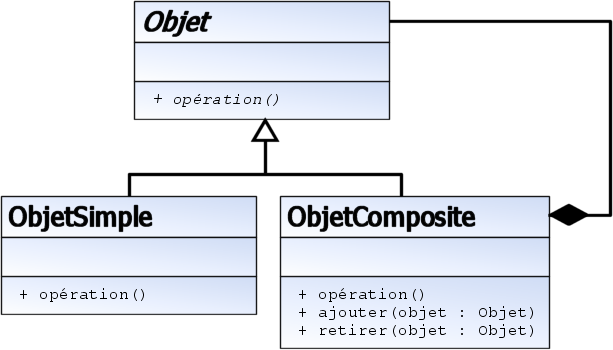
\includegraphics[height=4cm]{images/composite.png}
  \end{center}

  Dans notre code chaque agent planète a connaissance de ses voisins, sachant que ses voisins peuvent être soit des planètes libres, soit des planètes colonisées. Dans le code ce patron apparaît ainsi:

  \begin{cppcode*}{gobble=4}
    class Virtual_planet
    {
    protected:
      std::vector<Virtual_planet* > neighbourhood_;
    };
  \end{cppcode*}
  Ce patron nous évite bien sûr de complexifier le code avec une classe \texttt{voisin} qui alourdirait grandement nos simulations.

  \subsection{Patron stratégie}
  \begin{center}
    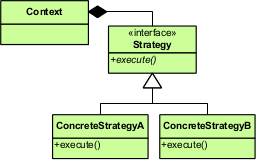
\includegraphics[height=4cm]{images/strategy.png}
  \end{center}

  Nous devons dans notre simulation traiter différemment nos agents en fonction de leur type, mais ceux ci doivent être stockés sur une même grille monde. De ce fait nous avons été obligés de recourir au patron stratégie. Dans le code, celui-ci apparaît de la manière suivante:

  \cppfile[firstline=38,lastline=44,label=Free\_planet.cpp,linenos=none]{../src/Free_planet.cpp}
  \cppfile[firstline=112,lastline=131,label=Colonized\_planet.cpp,linenos=none]{../src/Colonized_planet.cpp}
  Ce patron nous permet donc pour une même instruction, d’obtenir un comportement différent en fonction de l’agent activé.

  \subsection{Singleton}

  \begin{center}
    
\includegraphics[height=3cm]{images/single.png}
  \end{center}

  Comme expliqué précédemment nous avons décidé de rajouter une faction neutre à notre code mais celle-ci ne devait pas peser dans la mémoire de nos simulations. Nous en avons donc fait un singleton:
  \cppfile[firstline=13,lastline=22,label=Neutral\_faction.hpp,linenos=none]{../src/Neutral_faction.hpp}

  Il est à noter que pour terminer proprement le programme il faut appeler la méthode \texttt{dispose()} de ce singleton qui supprime proprement l’instance car le C++ ne vide pas automatiquement celle ci à la fin du programme.

  \section{Présentation des interfaces}

  Nous avons développé deux interfaces durant notre projet, la première en ASCII, qui nous a notamment permis de debugger le programme. Nous avons également implémenté une interface graphique, plus agréable à regarder et plus ergonomique. Cette implémentation nous a permis entre autres d’apprendre les rudiments de Qt.

  \subsection{Interface console}
  L’affichage en mode console est une méthode de l’objet monde. Elle affiche dans la sortie standard chaque case de la grille du monde ainsi que les statistiques des factions. Son code est le suivant:

  \cppfile[firstline=181,lastline=202,label=World.cpp,linenos=none]{../src/World.cpp}

  Le principe est simple: on parcourt chaque case de la grille monde et on appelle la méthode \texttt{display()} qui est une fonction surchargée suivant le patron stratégie. Ainsi les factions ont un caractère ASCII représentant leur capitale et un représentant leurs colonies. Si on appelle la méthode \texttt{display()} sur une colonie le caractère correspondant sera donné etc. Si la planète est libre la méthode renverra un simple point.
  A l’écran cette interface apparaît ainsi:
  \begin{center}
    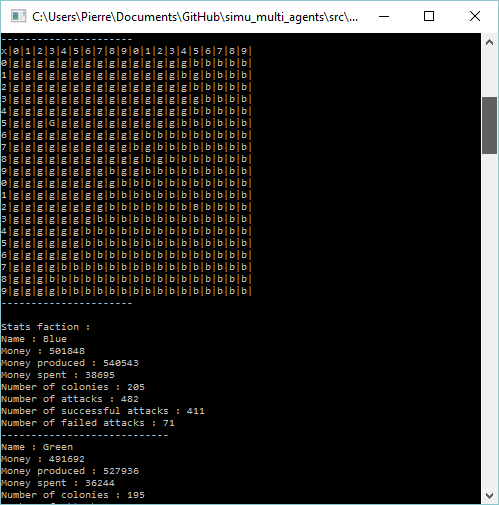
\includegraphics[height=12cm]{images/console.png}
  \end{center}


  \subsection{Interface Graphique}
  L’interface graphique faite sur Qt a pour avantage d’afficher plus de données que l’interface console et ce de manière plus claire. Elle possède elle aussi une fonction \texttt{display()} qui dessine les planètes et leurs statistiques quand celles-ci ont besoin d'être mises à jour (voir partie développement pour savoir comme l’afficheur détermine s’il doit redessiner une planète). L’afficheur graphique également met à jour les informations des factions en temps réel sur la droite de la fenêtre.
  
  Il permet également de distinguer les factions à l’aide d’une couleur et non plus d’un caractère. Ceci est dû au fait que chaque faction possède des champs \cppinline{color_colony} et \cppinline{color_motherland} qui sont les couleurs (\cppinline{string}) à donner aux fonctions de dessin de Qt pour obtenir certaines couleurs. Ainsi la fonction de Qt n’a qu’à appeler la méthode \cppinline{get_color()} (qui est aussi surchargée) sur chaque agent planète et ainsi les couleurs affichées seront celles liées aux factions. Si la planète est libre sa couleur sera par défaut le gris.
  
  Comme vu précédement, un champ \cppinline{change} nous permet de savoir si l’agent doit être redessiné. Si c’est le cas nous devons supprimer d’abord les anciens objets que nous avions dessiné. Pour cela, nous avons créé une classe \cppinline{QPlanet}, composée de pointeurs vers une ellipse, deux images et deux textes, que nous créons et supprimons au besoin. Ainsi nous évitons les fuites mémoire.
  
  A l’écran l’interface apparaît ainsi:
  \begin{center}
    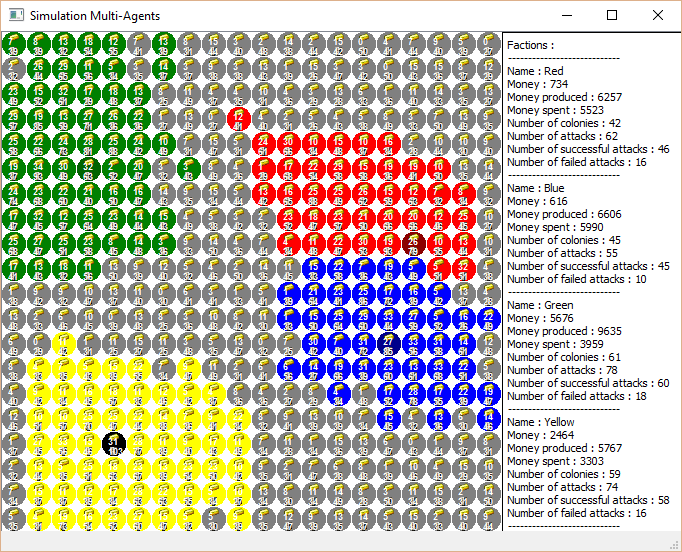
\includegraphics[height=12cm]{images/gui.png}
  \end{center}

  Le désavantage de cette interface est qu’elle ralentit beaucoup la simulation.

  Source des images: \href{https://fr.wikipedia.org}{\texttt{https://fr.wikipedia.org}}

  
  \chapter{Conclusion}

    La réalisation de ce projet nous a permis d'acquérir plus de pratique du C++, et d'apprendre à penser un programme en équipe. Egalement, la répartition du travail a eu son importance, et l'écriture d'un diagramme de Gantt nous a permis de jalonner toute la période de développement de différents repères afin de mener à bien la réalisation de ce projet, et de minimiser le nombre de bugs à corriger.

    Nous sommes satisfaits de notre travail, même si nous aurions souhaité produire un programme encore plus abouti en termes de paramètres ajustables pour la simulation.

    Nous avons été confrontés à différents problèmes lors du développement, notamment pour garantir l'"étanchéité" de la mémoire (Suppression du singleton, suppression des planètes remplacées lors des attaques...). D'autres problèmes se sont présentés lors de la suppression des planètes colonisés n'ayant pas encore joué, nous devions supprimer toutes leurs demandes de fonds pour empêcher des erreurs de segmentation qui arrivaient bien plus tard dans l'exécution et c'est pourquoi elles ont été difficiles à détecter. 
    Nous avons à plusieurs reprises été victimes d’une erreur lors de suppression d’un objet pointé par un itérateur qui parcourait un conteneur. En effet, la méthode erase(iterator) retourne un itérateur sur l’objet suivant celui qui est supprimé dans le conteneur, or nous ne récupérions pas cette valeur, et ainsi cela provoquait une erreur de segmentation au tour de boucle suivant.

    Nous avons été sensibles à la qualité du travail attendu, c’est pourquoi nous avons apporté beaucoup de soin dans le codage et la documentation de notre programme. Dans cette optique nous avons aussi proposé plusieurs exemples de simulation, à 2, 3 et 4 factions afin d’en observer le comportement et ainsi pouvoir ajuster certains paramètres (parfois borner certaines valeurs) de manière à obtenir des résultats plus réalistes.
    
    Enfin, nous avons revu notre diagramme de Gantt initial pour finalement respecter celui présenté ci-après, plus réaliste compte-tenu de la quantité de travail à fournir.

    \begin{center}
        \begin{ganttchart}[vgrid,hgrid]{1}{10}
\gantttitle{Séances}{10} \\
\gantttitlelist{1,...,10}{1} \\
\ganttgroup{Conception de base}{1}{5} \\
\ganttbar{Création de la grille "Monde"}{1}{1} \\
\ganttbar{Création des agents de base}{1}{1} \\
\ganttbar{Tirage des agents à exécuter}{2}{2} \\
\ganttbar{Planète mère et colonies}{3}{5} \\
\ganttbar{Faction}{3}{5} \ganttnewline
\ganttgroup{Simulation}{5}{9} \\
\ganttbar{Création du système économique}{5}{6} \\
\ganttbar{Création des désirs des factions (ordres etc)}{7}{9} \ganttnewline
\ganttgroup{Bonus !}{9}{10} \\
\ganttbar{Spécialisation de faction}{9}{9} \\
\ganttbar{Interface graphique}{10}{10}
\end{ganttchart}
    \end{center}

    \vfill 
    Notre code source est disponible sur la plateforme GitHub à l'adresse :
    \begin{center}
      \href{https://github.com/theCmaker/simu\_multi\_agents}{https://github.com/theCmaker/simu\_multi\_agents}
    \end{center}
    \vfill \null
  
  \appendix
  \chapter{Utilisation de Git}
Présentation réalisée par Pierre CHEVALIER.
\section{Résumé}
Git est un logiciel de gestion de versions décentralisé et libre développé notamment par Linus Torvalds et Junio Hamano. Il nous a permis de gérer les versions du projet conjointement avec le service d’hébergement de fichiers en ligne Github. Nous aurions également pu utiliser Git Server pour héberger nous-même les fichiers. Comme ce serveur aurait dû être lancé 24h/24 (car nous travaillions 24h/24) nous avons préféré utiliser une plateforme d’hébergement moins contraignante.

\noindent Les avantages notables de Git sont:
\begin{itemize}
	\item Chaque objet enregistré possède un identifiant universel en SHA1 qui permet de l’identifier de manière unique,
	\item Git est multi-protocole, ce qui signifie que les échanges peuvent se faire en ssh, http(s) etc,
	\item Les objets stockés sont compressés,
	\item Pas de relation client/serveur,
	\item Gestion efficaces des branches de développement.
\end{itemize}

Il peut être utilisé directement depuis un terminal, ce que nous faisions lorsque nous travaillions sur les terminaux de l’ISIMA, mais peut aussi être utilisé par d’autre logiciel  sous forme de plugin ou de programme dédié. Lors de développement du projet, nous avons notamment utilisé le logiciel de Github, Github Desktop, très utile dans le cadre d’une utilisation de Git sous Windows et non sous Linux ainsi que sous la forme d’un plugin intégré à Visual Studio.

Ces logiciels et plugin permettent une utilisation plus intuitive de Git, améliorant la vitesse de certaines actions prise par l’utilisateur.
\newpage
\noindent Quelques mots de vocabulaire:

\noindent
\begin{tabular}{p{0.1\textwidth}p{.85\textwidth}}
	Version & 
	On appelle version l’état du projet actuel, les fichiers présents, leur contenu etc. Git est un logiciel qui conserve toutes les versions enregistrées. \\
	
	Repository &
	Le répertoire. Dans ce rapport nous appellerons repository le répertoire git composé de toutes les versions enregistrées du projet. Le repository local est l’arborescence de version présente sur le disque dur de l’utilisateur, le repository distant est l’arborescence présente sur le serveur git. Lors d’un push ou d’un pull (d’un envoie de version ou une récupération de la version distante), les deux repositories se synchronisent. \\

	Commit &
	C’est un objet git (voir plus bas). On commit nos fichiers après une modification pour les enregistrer localement puis on les push pour envoyer les modifications au serveur.\\

	Branche &
	Une branche est une version de l’arborescence du projet. C’est-à-dire une mutation du projet avec ces propres versions. Elle permet notamment d’éviter les conflits récurrents lorsque deux développeurs travaillent sur des fichiers communs. Cette pratique part du principe de préféré faire une grosse fusion de la branche à la fin du développement plutôt que de faire une multitude de petites fusions à chaque fois qu’un des développeurs poste sur le repository distant. \\
	
	Clone &
	Un utilisateur de git peut cloner un repository. Git va copier toute l’arborescence du projet sur le disque dur de l’utilisateur. Celui-ci pourra ensuite envoyer ses propres commits sur le serveur distant s’il en a la permission. L’utilisateur peut aussi créer un nouveau repository en ligne basé sur cet ancien repository qu’il vient de cloner. \\

	Index &
	L’index est la dernière modification enregistrée par git (le dernier commit). Quand il faut envoyer les commit au repository distant, git va d’abord vérifier que son index est à jour avant d’envoyer. \\
	
	Conflit &
	Lorsque deux utilisateurs travaillent sur un même fichier, qu’ils le commit en même temps, il arrive que ces modifications soient issues d’une même version et donc lors de la mise à jour de repository distant (ou local si l’utilisateur n’a pas récupérer la dernière version enregistrée par le serveur distant) l’utilisateur peut être confronté à un conflit de fichier. Pour le résoudre, l’utilisateur peut choisir de conserver sa version locale ou la version distante ou encore faire une fusion des deux fichiers (il choisit quelles lignes conserver)
\end{tabular}

\section{Procédure d’installation}

Pour installer git sous un terminal il suffit  d’utiliser la commande suivante dans un terminal:
\begin{minted}{bash}
$ apt-get install git
\end{minted}

Si vous êtes sous Fedora, il faut utiliser la commande:
\begin{minted}{bash}
$ yum install git
\end{minted}

\noindent Tentez alors de lancer la commande \texttt{\$ git} pour vous assurer de la bonne installation du logiciel.

Si vous voulez également utiliser le service de cloud de Github, vous devez vous inscrire sur le site.

Pour installer Github Desktop il faut télécharger l’installateur à l’adresse suivante. Suivez les instructions et installer le logiciel. Celui-ci vous permettra d’installer de surcroit git sur votre ordinateur sous Windows en plus du logiciel Github Desktop.

Pour installer le plugin git sous Visual Studio il faut télécharger le plugin puis l’installer. Celui-ci vous permettra d’installer de surcroit git sur votre ordinateur sous Windows.

\section{Présentation des fonctionnalités}

Les logiciels de gestion de versions utilisent une arborescence de fichier permettant de conserver toutes les versions des fichiers et de mutualiser le développement entre les différents utilisateurs. Les développeurs mettent ainsi en ligne leur avancement accompagné d’un commentaire et le code source est mis à jour en fonction de cet avancement. Seuls les fichiers modifiés seront mis à jour. Un des avantages de ces logiciels est donc qu’ils limitent les doublons de données dans un projet qui peut être lourd en espace disque. Un autre avantage de ces logiciels est qu’ils permettent de gérer les conflits de version lorsque deux développeurs mettent leur avancement en ligne en même temps: une interface permet au dernier utilisateur qui a envoyé son travail de choisir quelles lignes garder.

Git se divise en deux structures de données: la base d’objets et le cache de répertoire. La base d’objet se trouve sur le disque dur client et se met à jour sur le serveur à chaque émission de versions et permet d’accéder à toutes les versions du projet alors que le cache de répertoire est uniquement sur la machine de l’utilisateur.

\noindent La base d’objet se compose de quatre types d’objet:
\begin{itemize} 
	\item         L’objet blob (binary large objects) qui correspond à une version d’un fichier
	\item         L’objet tree qui contient des objets blob comme un répertoire le ferait
	\item         L’objet commit qui donne accès à une arborescence (à un tree racine et vers ses commit parents). Il possède également un message de log.
	\item         L’objet tag qui est un message lié à un objet commit
\end{itemize}

Les actions possibles de l’utilisateur permettent d’ajouter et de supprimer ces objets.

Ces objets sont stockés dans le répertoire caché .git (situé dans le cache de répertoire). Le répertoire .git contient également des fichiers de configuration de l’environnement git, des informations sur les branches locales du repository, des logs, des infos sur l’état du prochain commit ...

\subsection{Git dans le terminal}
Le logiciel Git sous terminal consiste en une multitude de commandes permettant de créer des répertoires git, de récupérer les mises à jour distantes et d’exporter les mises à jour locales. Voici la liste des commandes les plus utilisées durant le projet et leur explication.

\noindent Commandes les plus utilisées:
\begin{itemize}
\item \textbf{git init:} Permet d’initialiser un repository sur le disque dur. Il va ainsi créer le .git d’un nouveau projet.
\item \textbf{git clone:} Permet de créer une copie d’un repository existant en ligne. L’utilisateur a alors accès à ce repository et peut même faire des commit (si cette utilisateur est autorisé par le serveur)
\item \textbf{git add:} Ajoute des fichiers de l’index du repository courant
\item \textbf{git rm:} Supprime des fichiers de l’index du repository courant
\item \textbf{git commit:} Prends tout les changements de l’index et crée un nouvel objet commit et sauvegarde cet objet en local. Un commentaire doit être associé à cet objet. Cette commande met à jour l’index du repository .
\item \textbf{git status:} Montre les différences qu’il y a entre le répertoire réel et l’index de repository. Il va lister les fichiers non enregistrés dans l’index, les fichiers modifiés et les fichiers prêts à l’envoie (c’est-à-dire dont la version a été enregistrée dans un objet commit)
\item \textbf{git branch:} Liste les branches existantes sur le projet. Crée une nouvelle branche si un nom est donné en argument.
\item \textbf{git checkout:} Permet de changer de branche.
\item \textbf{git merge:} Permet de fusionner deux branches. Cette action va automatique créer un nouveau commit s’il n’y a pas de conflits. Dans l’autre cas l’utilisateur va être invité à opérer à une fusion de fichiers ou à conserver une version.
\item \textbf{git reset:} Permet de retourner à la version du dernier objet commit crée (version de l’index).
\item \textbf{git pull:} Permet de récupérer les fichiers sur le repository distance vers le repository local. Equivalent à git fetch
\item \textbf{git push:} Permet d’envoyer les objets commit locaux au repository distant.
\item \textbf{git log:} Montre la liste des commit de la branche courante et les détails correspondants (les tags et les lignes modifiées par exemple)
\item \textbf{git show:} Montre les détails des commits locaux
\end{itemize}
\noindent Autres commandes:
\begin{itemize}
\item \textbf{git config:} Permet de configure le nom, l’email, etc de l’utilisateur
\item \textbf{git stash:} Sauvegarde des modifications que l’on ne veut pas commit immédiatement. Les changements pourront être appliqués plus tard.
\item \textbf{git tag:} Lie un message (un objet Tag) à un commit.
\item \textbf{git fetch:} Permet de récupérer les fichiers sur le repository distant vers le repository local
\item \textbf{git remote:} Montre toutes les versions distantes du repository
\item \textbf{git ls-tree:} Montre l’objet tree en incluant le nom de chaque objets et leur valeur en SHA-1
\item \textbf{git cat-file:} Prend en argument la valeur en SHA-1 d’un objet et permet de voir un objet
\item \textbf{git grep:} permet de faire une recherche à partir d’un mot clef dans un objet tree
\item \textbf{git diff:} Affiche les différences entre les modifications de l’index et celle du répertoire courant
\end{itemize}
L’avantage de cette interface commande est qu’elle permet une grande marge de manœuvre à l’utilisateur puisque celui-ci à accès à l’ensemble des commandes git et donc à un contrôle total de son repository. L’inconvénient le manque d’intuitivité de certaine commande.

\subsection{Git avec Github Desktop}

Github Desktop est un logiciel fournit par Github mais qui peut également être utilisé sur des plateformes d’hébergement autres que Github puisque l’installation du logiciel donne aussi accès à une interface en ligne de commande de Git, donnant accès de ce fait à toutes les commandes Git. On peut ainsi cloner des repositories sur des serveurs externes à Github tout en profitant quand même de l’interface graphique.

\begin{center}
	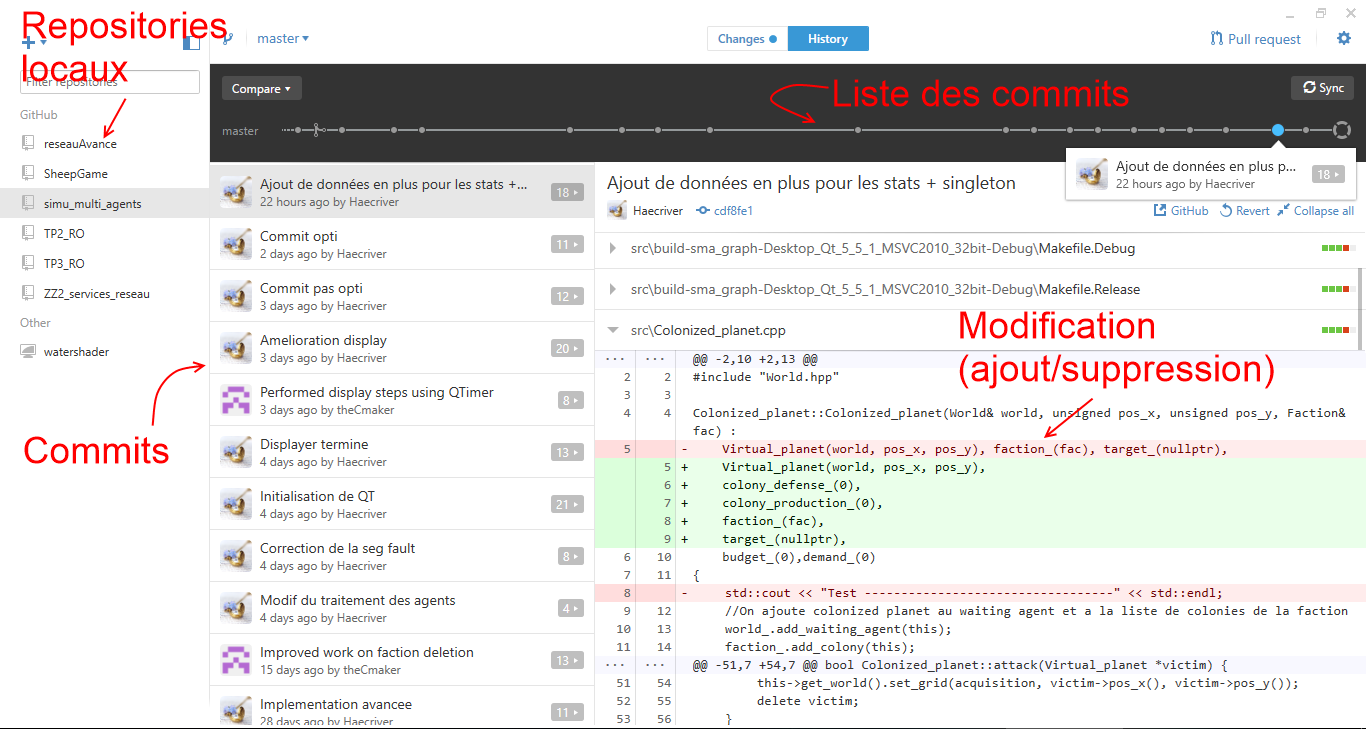
\includegraphics[width=\textwidth]{images/commit.png}
\end{center}
 
Celle-ci possède des capacités plus limité que l’interface commande. Par exemple on ne peut pas cloner un directement depuis l’interface graphique un  repository d’un serveur git distant (qui n’est pas Github) mais en contrepartie les merges sont plus intuitifs et la présentation des branches et commit est plus ergonomique.

\subsection{Git avec Visual Studio}

Le plugin de Visual Studio, tout comme le logiciel Github Desktop n’est pas aussi puissant que l’interface commande mais permet d’afficher l’historique des commits et surtout possède une interface facilitant grandement les merges si bien que nous n’avons pas eu besoin de travailler sur des branches durant le projet (sachant que celui-ci était réduit par rapport à de vrais projets professionnels bien entendu).

L’interface se présente ainsi:

\begin{center}
	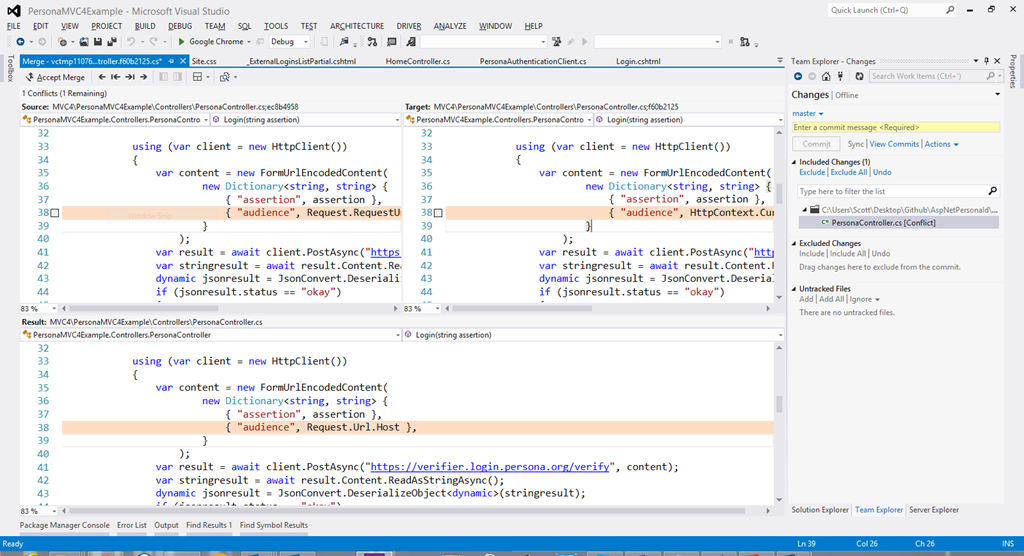
\includegraphics[width=.8\textwidth]{images/visual.png}
\end{center}

Visual présente les deux versions en conflit avec une case à cocher pour savoir quelle version conserver. Le résultat est affiché en dessous des deux fenêtres. Un bouton permet de passer rapidement au conflit suivant. S’il y a un problème ambigu, l’utilisateur peut toujours modifier le résultat à la main.
 
\noindent Références:\\
\href{https://git-scm.com/}{\texttt{https://git-scm.com/}}\\
\href{http://igm.univ-mlv.fr/~dr/XPOSE2008/git/fonctionnement.html}{\texttt{http://igm.univ-mlv.fr/~dr/XPOSE2008/git/fonctionnement.html}}\\
\href{https://www.siteground.com/tutorials/git/commands.htm}{\texttt{https://www.siteground.com/tutorials/git/commands.htm}}\\
\href{https://fr.wikipedia.org/wiki/Git}{\texttt{https://fr.wikipedia.org/wiki/Git}}\\
\href{https://fr.wikipedia.org/wiki/GitHub}{\texttt{https://fr.wikipedia.org/wiki/GitHub}}

\noindent Image merge visual:\\
\href{http://www.hanselman.com/blog/content/binary/Windows-Live-Writer/ed5b594103c4\_B6D0/image\_2.png}{\texttt{http://www.hanselman.com/blog/content/binary/Windows-Live-Writer/ed5b594103c4\_B6D0/image\_2.png}}
  \chapter{Doxygen -- Présentation d'un outil de documentation}
Présentation réalisée par Pierre-Loup PISSAVY.
\section{Présentation}

  Doxygen est un outil permettant de générer automatiquement de la documentation à partir de code source. Ceci est possible grâce à l'implantation de balises particulières dans les commentaires présents dans le code.
  C'est un outil qui supporte plusieurs langages, et parmi les plus connus, le C/C++ et Java. La documentation ainsi produite peut alors être publiée, imprimée ou simplement sauvegardée.

  Cela permet à la fois de produire de la documentation et de renseigner le développeur sur le code qu'il consulte. La documentation étant présente dans le code, cela permet de la garder à jour (un seul fichier à modifier pour mettre à jour la documentation), et facile à compléter.

\section{Installation}
\subsection{Logiciel}
  Doxygen est d'une grande flexibilité, l'outil est disponible sur toutes les plateformes communes: Windows, Mac OS X, et les systèmes Unix (BSD, GNU/Linux).

  Sur les systèmes Unix, il est présent dans les dépôts officiels de paquets orientés développement, on peut donc utiliser notre gestionnaire de paquets préféré, par exemple:
  \begin{minted}[gobble=4]{bash}
    yum install doxygen
  \end{minted}

  Pour les systèmes Windows et Max OS X, on peut télécharger les installateurs sur le site officiel de Doxygen,
  \href{http://www.doxygen.org/download.html}{\texttt{http://www.doxygen.org/download.html}},
  ou bien sur le dépôt GitHub officiel (\href{https://github.com/doxygen/doxygen}{\texttt{https://github.com/doxygen/doxygen}})
  si l'on souhaite obtenir ou tester les derniers changements.

\subsection{Plug-ins}
  Doxygen est l'un des outils de documentation les plus connus, aussi l'on trouve de nombreux plugins afin de l'intégrer au sein des IDE les plus utilisés. C'est le notamment le cas d'Eclipse, NetBeans, QtCreator, MS VisualStudio et XCode.

\section{Fonctionnalités proposées}
  Pour chaque document à produire, Doxygen nécessite un fichier de configuration, usuellement nommé \emph{Doxyfile}\footnote{Par référence au Makefile de l'outil Make}. Ce fichier de configuration contient de très nombreux paramètres, et sa trame peut être générée automatiquement avec la commande 
  \begin{minted}[gobble=4]{bash}
    doxygen -g
  \end{minted}

  Pour construire la documentation, on exécute simplement dans le dossier contenant le Doxyfile la commande suivante:
  \begin{minted}[gobble=4]{bash}
    doxygen
  \end{minted}

  Tous les paramètres de configuration sont comparables à des variables du shell et la syntaxe en est très proche.

  Doxygen fait précéder chaque variable de commentaires expliquant son emploi et parfois les propriétés à respecter.
  
  \subsection{Réglage du rendu}
    \noindent
    \begin{tabular}{p{.25\linewidth}p{.7\linewidth}}
      \texttt{PROJECT\_NAME} & Le nom du projet. \\
      \texttt{PROJECT\_NUMBER} & La version de la documentation ou du projet selon ce que l'on souhaite. \\
      \texttt{PROJECT\_BRIEF} & Une brève description du projet. \\
      \texttt{PROJECT\_LOGO} & Le chemin (relatif ou absolu par rapport au Doxyfile) d'une image ou logo représentant le projet (dimensions conseillées 200 $\times$ 50 px). \\
      \texttt{OUTPUT\_DIRECTORY} & Le dossier dans lequel la documentation doit être produite (celui du Doxyfile par défaut). \\
      \texttt{OUTPUT\_LANGUAGE} & La langue dans laquelle la documentation est produite (cela permet de faire correspondre le fond et la forme du résultat).
    \end{tabular}

  \newpage
  \subsection{Réglage de l'extraction de documentation}
    A l'exception des deux dernières, toutes les variables qui suivent sont booléennes et peuvent prendre la valeur \texttt{YES} ou \texttt{NO}.\\

    \noindent
    \begin{tabular}{p{.3\linewidth}p{.65\linewidth}}
      \texttt{EXTRACT\_ALL} & Impose à Doxygen de vérifier que toutes les classes ont été documentées.\\
      \texttt{EXTRACT\_PRIVATE} & Extrait la documentation des membres privés dans les classes.\\
      \texttt{EXTRACT\_STATIC} & Extrait la documentation des membres statiques.\\
      \texttt{EXTRACT\_LOCAL\_CLASSES} & Extrait la documentation des classes imbriquées ou déclarées localement.\\
      \texttt{HIDE\_UNDOC\_MEMBERS} & Enlève du document final les membres qui ne sont pas documentés.\\
      \texttt{RECURSIVE} & Inspecte également la sous-arborescence à la recherche de fichiers comportant de la documentation.\\
      \texttt{EXCLUDE} & Liste des fichiers et/ou répertoires à exclure de la recherche de documentation.\\
      \texttt{FILE\_PATTERNS} & Schémas des noms de fichiers qui peuvent être inspectés\footnotemark[2].\\
    \end{tabular}
    \footnotetext[2]{Par défaut, Doxygen reconnaît les extensions usuelles, cette variable permet de sélectionner uniquement les extensions que l'on souhaite, et de les personnaliser}

  \subsection{Et dans le code...}
    En C++, la fragmentation entre déclaration et définition pourrait présenter un frein à la documentation (où documenter, comment éviter les répétitions ?), mais Doxygen reconnaît aussi bien les commentaires dans les headers que dans les fichiers source. Cela permet de documenter les classes, membres et méthodes simples (getters/setters) directement dans le header, et de documenter les méthodes et fonctions détaillées dans les fichiers source.


    La documentation se fait donc dans des commentaires dont le formatage est spécial (il reprend les commentaires classiques du C++, en ajoutant simplement un caractère distinctif permettant de signaler le contenu comme de la documentation). Dans le cas du C/C++, cela peut-être un troisième caractère \texttt{'/'} pour les commentaires sur une ligne, ou bien l'ajout d'une étoile (\texttt{*}) sur la balise ouvrante des commentaires multiligne.

    En voici un exemple:
    \begin{cppcode*}{gobble=6}
      /**
       * @class Personne
       * @brief Classe représentant une personne à l'aide de quelques informations de base
       * 
       * Informations plus détaillées
       */
      class Person {
        private:
          std::string first_name_;  ///< Prénom
          std::string family_name_; ///< Nom de famille
          Date        birthdate_;   ///< Date de naissance
          Gender      gender_;      ///< Sexe
      };
    \end{cppcode*}

    Nous pouvons voir à travers cet exemple que les informations sont indiquées de manière sémantique. En effet, Doxygen nécessite l'emploi de balises afin de caractériser le type de l'information apportée.

    \newpage
    Ces balises sont généralement précédées indifféremment du symbole \texttt{@} ou \texttt{\textbackslash}.

    Voici une liste non exhaustive des plus usitées:

    \noindent
    \begin{tabular}{p{.2\textwidth}p{.7\textwidth}}
      \texttt{@file}   & Nom du fichier.\\
      \texttt{@author} & Auteur(s).\\
      \texttt{@details} & Détails.\\
      \texttt{@version} & Version du fichier.\\
      \texttt{@date}    & Date ou intervalle de dates fixes.\\
      \texttt{@bug}     & Pour signaler un comportement inattendu (permet de créer une liste de bugs).\\
      \texttt{@warning} & Pour signaler les conditions d'utilisation à respecter.\\
      \texttt{@copyright} & Licences.\\ 
      \texttt{@see} & Référence vers un autre élément en relation avec celui portant la balise.\\
      \texttt{@deprecated} & Elément obsolète.\\
      \texttt{@note} & Information sur le comportement ou à destination des autres développeurs.\\
      \texttt{@param} & Suivi du nom d'un paramètre et de sa description, pour décrire les paramètres d'une méthode/fonction. \\
      \texttt{@pre} & Préconditions. \\
      \texttt{@post} & Postconditions. \\
      \texttt{@remark} & Remarques. \\
      \texttt{@return} & Valeur retournée. \\
    \end{tabular}

    \noindent
    \begin{tabular}{p{.2\textwidth}p{.7\textwidth}}
      \texttt{@since} & Pour signaler depuis quand ou quelle version l'élément est disponible. \\
      \texttt{@todo} & Choses restant à faire (une liste peut être constituée à partir de ces balises). \\
      \texttt{@struct} & Description de structure en C/C++.\\
      \texttt{@class} & Description de classe en C/C++.\\
      \texttt{@a} & Suivi du nom d'un paramètre/argument, fait référence à un argument.
    \end{tabular}

    L'utilisation de Qt permet également de remplacer les symboles additionnels énoncés plus haut par des points d'exclamation (pour correspondre au style Qt). C'est ce que nous avons choisi dans notre projet (QtCreator pré-remplit les commentaires de documentation).

    Dans les commentaires courts comme pour décrire le prénom, le chevron ouvrant remplace la balise \texttt{@brief}.

    Enfin, il est possible de présenter la documentation de manière structurée en employant des listes de la même manière que dans un wiki, ou bien en utilisant directement du code HTML pour les compositions plus complexes.

\section{Utilisation au sein du TP Multi-agents}
  Doxygen nous a permis d'obtenir une documentation dont la présentation est agréable et peut être rendue accessible à tous. Cela est possible en publiant la version web HTML ou bien en diffusant le PDF qui peut être généré à partir des fichiers source \LaTeX{} produits par Doxygen.

  Nous avons ajouté le logo de l'école et quelques informations sommaires sur le projet.

  Il est bien évidemment possible de produire une documentation encore plus étoffée et consistante, mais cela demande toujours beaucoup de temps, tant du point de vue de la rédaction/mise en forme, que des revirements de situation dans le développement des objectifs à atteindre.

\section{En bref}
  Pour résumer, Doxygen est un outil très complet permettant une documentation efficace et sémantique du code. Il présente le gros avantage d'être utilisable sur plusieurs plateformes, avec plusieurs langages et d'obtenir plusieurs formats de sortie, de la version Web aux pages de manuel en passant par l'incontournable PDF. 

  Sa renommée lui vaut l'existence de plug-ins pour les plus grands environnements de développement, ce qui n'est pas négligeable (auto-complétion, pré-documentation...) lorsqu'il s'agit de gagner du temps.

  Les possibilités sont très étendues, et encore trop peu exploitées, c'est un outil qui mérite d'être promu auprès des développeurs (jeunes et senior) afin de rendre le développement et la maintenance de projets plus efficaces.

\section*{Sources d'information}
  \begin{itemize}
    \item Site officiel de Doxygen: \\
    \href{http://www.doxygen.org/}{\texttt{http://www.doxygen.org/}}
    \item Initiation à Doxygen:\\
     \href{http://franckh.developpez.com/tutoriels/outils/doxygen/}{\texttt{http://franckh.developpez.com/tutoriels/outils/doxygen/}}
    \item Using Doxygen: \\
    \href{http://lugatgt.org/2002/05/30/using-doxygen/}{\texttt{http://lugatgt.org/2002/05/30/using-doxygen/}}
    \item Plug-in pour QtCreator:\\
    \href{http://dev.kofee.org/projects/qtcreator-doxygen/wiki}{\texttt{http://dev.kofee.org/projects/qtcreator-doxygen/wiki}}
    \item 10 Minutes to document your code:\\ 
    \href{http://www.codeproject.com/Articles/3528/Minutes-to-document-your-code}{\texttt{http://www.codeproject.com/Articles/3528/Minutes-to-document-your-code}}
  \end{itemize}

  \chapter{Résultats}
Ces résultats, bien que non utilisables puisque notre simulation a été créée avec des valeurs empiriques permettent toutefois de quantifier les valeurs et les probabilités liées aux agents de la simulation.

Les significations des cases sont les suivantes:

\begin{itemize}
\item Death : Nombre de tours avant la mort de la faction
\item Money : Argent à la mort de la faction
\item Prod : Argent produit par la faction
\item Spent : Argent dépensé par la faction
\item Nb colonies : Nombre de colonies à la mort de la faction
\item Nb attacks : Nombre d’attaques exécutées par la faction
\item Nb success : Nombre d’attaque réussies
\item Nb fails : Nombre d’attaques échouées\\

\item ML x : Position x de la planète mère de la faction
\item ML y : Position x de la planète mère de la faction
\item ML natdef : Défense naturelle de la planète mère (à l’inititialisation)
\item ML natprod : Production naturelle de la planète mère (à l’inititialisation)
\item ML findef : Défense finale de la planète mère
\item ML finprod : Production finale de la planète mère
\end{itemize}

\section{Résultats de cent simulations avec deux factions}
\subsection{Moyenne faction gagnante}

\begin{tabular}{|c|c|c|c|c|c|c|c|}
	\hline Death & Money & Prod & Spent & Nb colonies & Nb attacks & Nb success & Nb fails \\ 
	\hline 1028,34 & 156366,954 & 236889,458 & 180007,563 & 240,73 & 6251,58 & 5596,68 & 654,9 \\
	\hline
\end{tabular}

\begin{tabular}{|c|c|c|c|c|c|}
	\hline ML x & ML y & ML natdef & ML natprod & ML findef & ML finprod \\ 
	\hline 8,96 & 9,47 & 38,16 & 8,27 & 89,56 & 25,39 \\
	\hline
\end{tabular}

\subsection{Moyenne autres factions (éliminées)}

\begin{tabular}{|c|c|c|c|c|c|c|c|}
	\hline Death & Money & Prod & Spent & Nb colonies & Nb attacks & Nb success & Nb fails \\ 
	\hline 1026,34 & 131796,532 & 134702,934 & 156382,954 & 82,48 & 6099,82 & 5487,23 & 612,59 \\
	\hline
\end{tabular}

\begin{tabular}{|c|c|c|c|c|c|}
	\hline ML x & ML y & ML natdef & ML natprod & ML findef & ML finprod \\ 
	\hline 9,29 & 10,01 & 37,98 & 6,54 & 88,55 & 23,79 \\
	\hline
\end{tabular}

\section{Interprétation}

En règle générale, il semble que les valeurs finales des factions gagnantes sont supérieures aux valeurs des factions vaincues.

Il est intéressant de noter que les défenses naturelles (défense à l’initialisation) des factions est un facteur qui a moins d’importance que la production naturelle (à l’initialisation) car si la moyenne du premier est environ égale à celle d’une faction gagnante contre une faction perdante, le deuxième lui est légèrement plus élevé pour la faction gagnante.

Un autre point important est qu’en moyenne la faction gagnante possède trois fois plus de colonies à la fin de la simulation que la faction perdante.
   
\end{document}
